\chapter{The Standard Model and CMS}


\section{The Standard Model of Particle Physics}

The Standard Model (SM) provides a comprehensive framework that connects the known fundamental particles to three of the four fundamental forces: the strong force, the weak force, and the electromagnetic force. It organises the elementary particles—specifically, the matter particles (quarks and leptons) and the force-carrying particles—under a unifying principle of symmetry. This symmetry ensures that the laws of physics remain consistent even as particles interact through these forces \cite{pich2012standardmodelelectroweakinteractions}.

In the SM, the strong force, which holds quarks together to form protons and neutrons, is carried by particles called gluons. The weak force, responsible for processes like radioactive decay, is mediated by particles known as the W and Z bosons. Meanwhile, the electromagnetic force, which controls how charged particles interact, is carried by the photon \cite{pich2012standardmodelelectroweakinteractions}. These forces are tied together through the SM’s symmetry, which helps explain why particles behave the way they do in nature.

The matter particles in the SM are divided into quarks and leptons. Quarks are the building blocks of protons and neutrons, while leptons include familiar particles like electrons and their neutral partners, neutrinos. These particles are arranged into three generations, each containing two quarks and two leptons (see figure \ref{fig:standard_model}). The first generation includes the lightest and most stable particles, such as the up and down quarks (which make up protons and neutrons) and the electron and its neutrino. The second and third generations contain heavier, less stable particles that quickly decay into first-generation particles. This repeating family structure explains why protons and neutrons are made of first-generation quarks, while heavier particles are short-lived \cite{cush:standard-model}.

\begin{figure}[h]
    \centering
    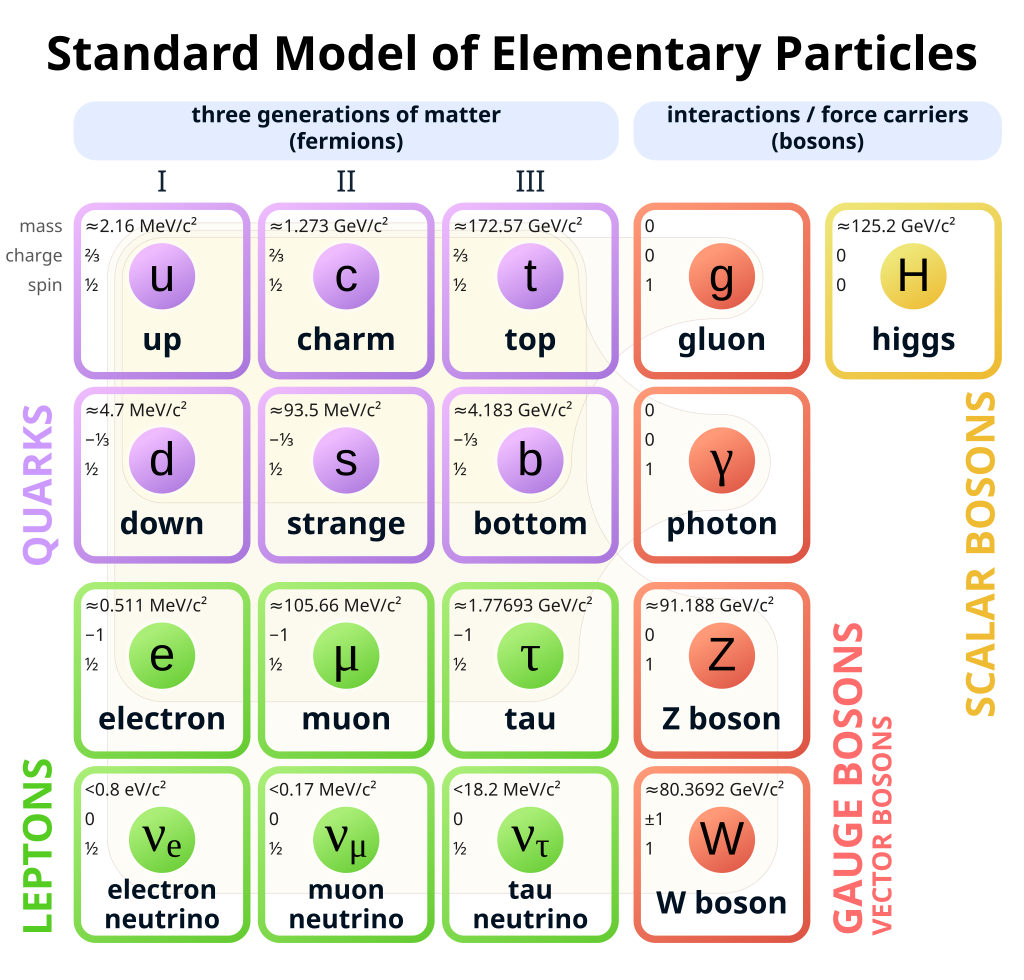
\includegraphics[width=0.75\linewidth]{media/1024px-Standard_Model_of_Elementary_Particles.svg.png}
    \caption{Standard model of elementary particles: the 12 fundamental fermions and 5 fundamental bosons \cite{cush:standard-model}.}
    \label{fig:standard_model}
\end{figure}

A key aspect of the SM is how it accounts for the masses of certain particles. While the symmetry of the SM keeps the photon massless, the W and Z bosons, which are involved in the weak force, need to have mass to match experimental observations. This happens through a process where the symmetry is hidden in the everyday world but still governs the underlying physics, known as spontaneous symmetry breaking \cite{pich2012standardmodelelectroweakinteractions}. The Higgs field, a field that fills all of space and was proposed in the 1960s by physicists like Englert, Brout, and Higgs, makes this possible. The Higgs field gives mass to the W and Z bosons and, in the process, predicts the existence of a new particle: the Higgs boson \cite{pich2012standardmodelelectroweakinteractions}.

For decades, the Higgs boson remained the missing piece of the SM. In 2012, experiments at CERN’s Large Hadron Collider (LHC), conducted by the ATLAS and CMS teams, discovered a new particle with a mass of about 125 GeV \cite{Chatrchyan_2012}. This particle’s properties have been studied extensively and align with the Higgs boson predicted by the SM, confirming the mechanism that gives mass to other particles  \cite{Chatrchyan_2012}.

Despite its success in explaining many experimental results, the SM is not a complete theory. It leaves several big questions unanswered. The SM does not explain why there are exactly three generations of particles, each with similar properties but different masses. It also originally assumed neutrinos had no mass, but by now it is known that they have tiny masses, meaning the model needs to be adjusted.
The SM does not solve the mystery of why the Higgs boson’s mass is so small compared to what quantum effects suggest either — a problem called the hierarchy problem. These gaps suggest the SM is just part of a bigger picture that has not been fully uncovered yet. To do so, particle accelerators are used to challenge the assumptions made in the SM and even go farther — or in this case smaller and into even higher energy scales — and try to look for physics beyond the SM.

\section{The Large Hadron Collider}

To explore phenomena at distance scales far below $10^{-18}$ m (i.e. at extremely high energy scales), physicists rely on high-energy particle collisions. The LHC at CERN is the world’s largest and most powerful particle accelerator, designed to probe such distance scales by colliding protons at unprecedented energies. It is a 27 km circumference circular accelerator that accelerates two counter-rotating beams of protons to nearly the speed of light and brings them into head-on collision at four interaction points. The LHC, whose design centre-of-mass energy is 14 TeV (7 TeV per beam) \cite{Evans:2008zzb}, was built to achieve a peak instantaneous luminosity of $1\times10^{34}$ cm$^{-2}$s$^{-1}$ \cite{Evans:2008zzb}. In its successful Run-1 (2010–2013) and Run-2 (2015–2018) operations, the LHC reached collision energies up to 13 TeV and even exceeded the design luminosity – achieving about $2\times10^{34}$ cm$^{-2}$s$^{-1}$ in 2018 \cite{Hayrapetyan_2024}. The machine is now in Run-3 (2022–present) with a slight energy increase (13.6 TeV). It is being upgraded for the High-Luminosity LHC (HL-LHC) era later this decade, which aims to further boost the luminosity by about an order of magnitude \cite{tomei2025cmsupgradeshighluminositylhc}.

\begin{figure}[h]
    \centering
    \includegraphics[width=0.9\linewidth]{media/CCC-v2018-print-v2.pdf}
    \caption{ Sketch of the CERN accelerator complex \cite{Mobs:2636343}.}
    \label{fig:lhc}
\end{figure}

Figure \ref{fig:lhc} shows the structure of the CERN complex with the LHC at its heart. On the discovery front, the LHC’s first triumphant success was the Higgs boson. Ongoing searches continue for signs of physics beyond the SM – for example, heavy supersymmetric particles, extra dimensions, or new force carriers – across many possible decay channels. So far, no clear evidence of new particles has appeared; extensive searches in the most promising channels have found no statistically significant deviations from SM expectations \cite{sonneveld2025susyhighlightscurrentresults}.

\section{The CMS Experiment}

Collision events in the LHC produce quarks and gluons that cannot exist as free particles (colour confinement \cite{pich2012standardmodelelectroweakinteractions}). Instead, the outgoing parton radiates additional quarks and gluons, forming a parton shower whose virtuality cascades down to $\mathcal{O}(\mathrm{GeV})$, where hadronisation binds them into colour-neutral hadrons. These hadrons emerge in a narrow cone around the original parton direction, forming a visible spray—a jet. 

The CMS detector is one of the two general-purpose detectors at the LHC designed to record these jets with high efficiency and precision, enabling a broad physics program from Higgs boson studies to searches for new phenomena. It is built in a layered, cylindrical geometry around the collision point (see figure \ref{fig:cms_overview}) and, despite the name "Compact", enormous in absolute terms: it is about 15~m in diameter, 21~m in length, and weighs about 14,000 tonnes. At the heart of CMS is a superconducting solenoid coil that generates a magnetic field of 3.8 T within a 6~m inner diameter. This bends the trajectories of charged particles, allowing their momenta to be measured; the steel structure that contains the magnetic flux (the return yoke) also serves as the absorber for muon detection and accounts for the bulk of CMS’s mass. Inside the magnet coil, CMS is packed with high-precision tracking and calorimetry systems, and outside the coil are large muon detector chambers, as shown in figure \ref{fig:cms_overview} \cite{CMS}.

\begin{figure}[h]
\centering
    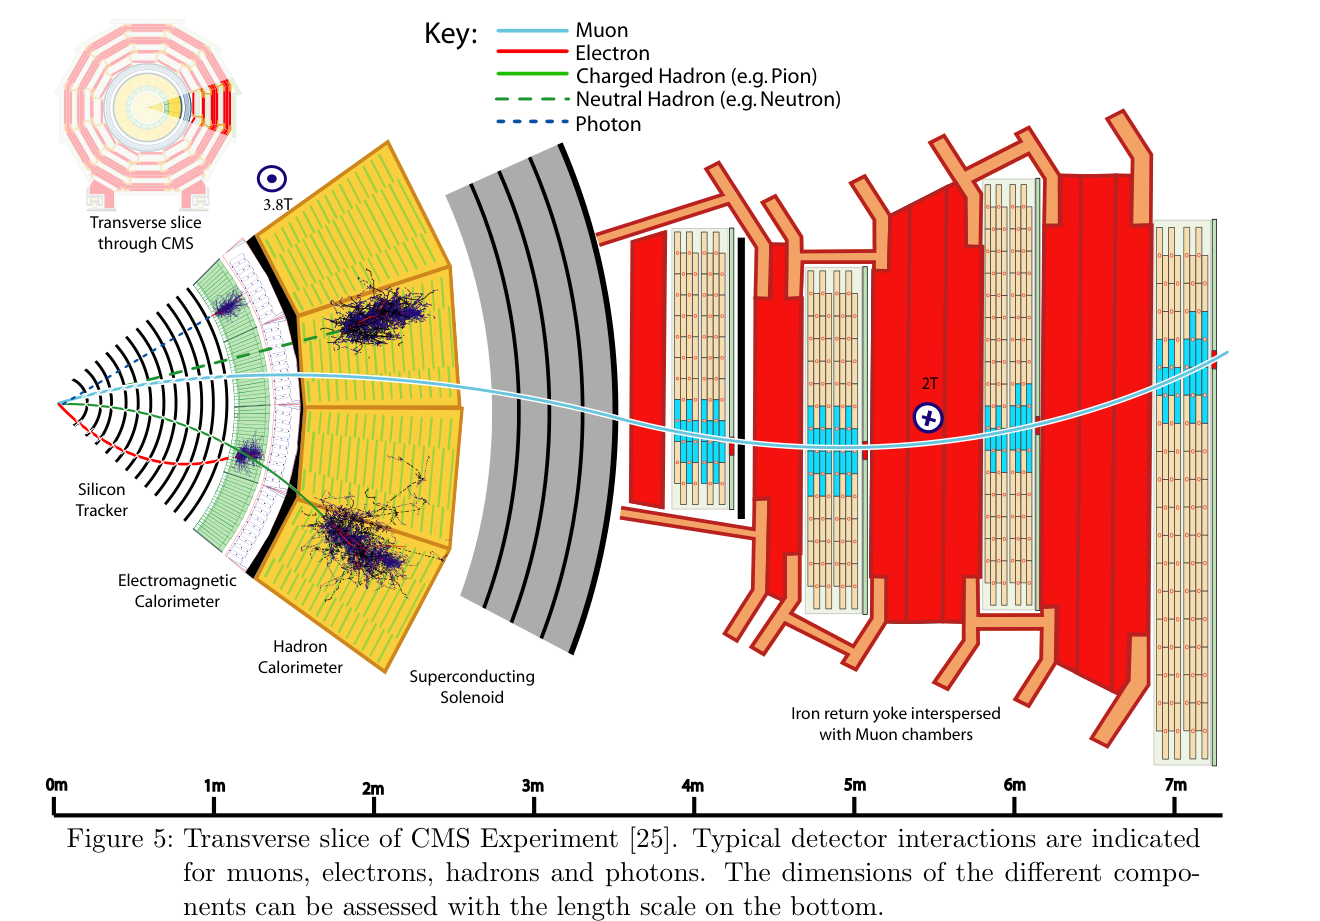
\includegraphics[width=15cm]{media/cms_cutview.png}
    \caption{Slice of the CMS Detector adapted from \cite{Sirunyan_2017}.}
    \label{fig:cms_overview}
\end{figure}
\newpage
Moving outward from the beam line, the first subsystem is the silicon tracker, a high-granularity detector made of about 75 million individual silicon strips and pixels arranged in concentric layers \cite{CMS}. When a charged particle from a collision passes through the tracker, it leaves hits in these silicon sensors. By reconstructing sequences of hits, CMS can trace out the tracks of charged particles with fine spatial resolution. The strong magnetic field bends these tracks; the particle’s momentum can be determined from the curvature. The tracker is designed to be extremely precise, allowing the reconstruction of secondary vertices from $b$-hadron decays a few centimetres from the collision point.

Surrounding the tracker is the electromagnetic calorimeter (ECAL), which is made of dense lead tungstate ($\text{PbWO}_4$) crystals. The ECAL’s task is to fully absorb and measure the energy of electrons and photons \cite{CMS}. When an electron or high-energy photon enters the ECAL, it initiates an electromagnetic shower in the crystal. The light output from the crystals is proportional to the particle’s energy. The CMS ECAL provides excellent energy resolution (on the order of 1\% for high-energy electrons/photons) and was pivotal in the Higgs boson discovery via the $H\to\gamma\gamma$ decay mode \cite{Chatrchyan_2012}.

Outside the ECAL lies the hadron calorimeter (HCAL). It is sampling calorimeter using alternating layers of absorber (brass or steel) and plastic scintillator. The HCAL is designed to stop and measure the energy of hadrons \cite{CMS}. Hadrons penetrate the ECAL but are largely absorbed in the thicker material of the HCAL, producing cascades of secondary particles. By collecting the scintillation light from these showers, the HCAL provides a measurement of the hadronic energy. Although the HCAL’s resolution is coarser than that of the ECAL, combining its information with the ECAL and tracker allows reconstruction of the energy and direction of jets as well as the estimation of missing transverse energy.

The outermost layers of CMS are the dedicated muon detectors, which give the experiment its name. Muons are charged leptons similar to electrons but about 200 times heavier, and they are penetrating: unlike most particles, muons can traverse substantial amounts of matter. In CMS, after passing through the calorimeters, muons still have enough energy to reach the muon chambers interleaved in the steel return yoke \cite{CMS}. CMS employs several types of muon detectors (drift tubes, cathode strip chambers, and resistive plate chambers) to track muons independently of the inner tracker. By matching muon tracks in the muon system with those in the inner tracker, CMS achieves a very accurate muon momentum measurement.

\subsection{Trigger System}
As the LHC collision rate is enormous, CMS cannot record data from every collision. Instead, the experiment uses a trigger system to filter events in real time. CMS employs a two-level trigger system: a Level-1 (L1) trigger implemented in custom electronics (fast hardware logic) and a High-Level Trigger (HLT) implemented in software running on a computing farm \cite{Khachatryan_2017}. The L1 trigger, which is using information from the calorimeters and muon system, reduces the 40 MHz collision rate to around 100 kHz by selecting events with interesting signatures (such as high-energy objects). Then the HLT takes those L1-selected events and runs a streamlined version of the full event reconstruction to apply more refined selection criteria, outputting a final rate of around 1 kHz to permanent storage \cite{Khachatryan_2017}. This multi-tiered trigger is crucial for ensuring that the most interesting collisions – those potentially containing rare new physics or useful signals – are recorded for offline analysis, while discarding the rest.

\subsection{Coordinates}
CMS uses a right-handed coordinate system with the origin at the centre of the detector. The x-axis points radially inward toward the centre of the LHC ring, the y-axis points vertically upward, and the z-axis is aligned with the beam direction \cite{Chatrychan_2008}. Instead of simple Cartesian coordinates $(x,y,z)$, it is often convenient to use cylindrical and spherical coordinates $(r,\phi,\theta)$ (or equivalently $(r,\phi,\eta)$) to describe angles and distances. Here, $r$ denotes the distance from the beam line in the transverse plane ($x$–$y$ plane), $\phi$ is the azimuthal angle in that plane (with $\phi=0$ defined along the positive x-axis), and $\theta$ is the polar angle measured from the positive $z$-axis.

In practice, the polar angle $\theta$ is expressed via the pseudorapidity $\eta$, defined as:

\begin{equation}
    \eta = - \ln \left( \tan \frac{\theta}{2}\right)
\end{equation}

For highly relativistic particles (with $E \gg m$), the pseudorapidity $\eta$ is approximately equal to the particle’s rapidity $y$, which is given by

\begin{equation}
    y = \frac{1}{2} \ln\frac{E+p_z}{E-p_z},
\end{equation}

where $E$ is the particle’s energy and $p_z$ is the $z$-component of the momentum; the transverse momentum is $p_T=\sqrt{p_x^2+p_y^2}$. This coordinate choice conveniently captures the detector’s cylindrical symmetry and the boost-invariant nature of motion along the beam axis \cite{Chatrychan_2008}.